\documentclass[twoside]{book}

% Packages required by doxygen
\usepackage{fixltx2e}
\usepackage{calc}
\usepackage{doxygen}
\usepackage[export]{adjustbox} % also loads graphicx
\usepackage{graphicx}
\usepackage[utf8]{inputenc}
\usepackage{makeidx}
\usepackage{multicol}
\usepackage{multirow}
\PassOptionsToPackage{warn}{textcomp}
\usepackage{textcomp}
\usepackage[nointegrals]{wasysym}
\usepackage[table]{xcolor}

% Font selection
\usepackage[T1]{fontenc}
\usepackage[scaled=.90]{helvet}
\usepackage{courier}
\usepackage{amssymb}
\usepackage{sectsty}
\renewcommand{\familydefault}{\sfdefault}
\allsectionsfont{%
  \fontseries{bc}\selectfont%
  \color{darkgray}%
}
\renewcommand{\DoxyLabelFont}{%
  \fontseries{bc}\selectfont%
  \color{darkgray}%
}
\newcommand{\+}{\discretionary{\mbox{\scriptsize$\hookleftarrow$}}{}{}}

% Page & text layout
\usepackage{geometry}
\geometry{%
  a4paper,%
  top=2.5cm,%
  bottom=2.5cm,%
  left=2.5cm,%
  right=2.5cm%
}
\tolerance=750
\hfuzz=15pt
\hbadness=750
\setlength{\emergencystretch}{15pt}
\setlength{\parindent}{0cm}
\setlength{\parskip}{3ex plus 2ex minus 2ex}
\makeatletter
\renewcommand{\paragraph}{%
  \@startsection{paragraph}{4}{0ex}{-1.0ex}{1.0ex}{%
    \normalfont\normalsize\bfseries\SS@parafont%
  }%
}
\renewcommand{\subparagraph}{%
  \@startsection{subparagraph}{5}{0ex}{-1.0ex}{1.0ex}{%
    \normalfont\normalsize\bfseries\SS@subparafont%
  }%
}
\makeatother

% Headers & footers
\usepackage{fancyhdr}
\pagestyle{fancyplain}
\fancyhead[LE]{\fancyplain{}{\bfseries\thepage}}
\fancyhead[CE]{\fancyplain{}{}}
\fancyhead[RE]{\fancyplain{}{\bfseries\leftmark}}
\fancyhead[LO]{\fancyplain{}{\bfseries\rightmark}}
\fancyhead[CO]{\fancyplain{}{}}
\fancyhead[RO]{\fancyplain{}{\bfseries\thepage}}
\fancyfoot[LE]{\fancyplain{}{}}
\fancyfoot[CE]{\fancyplain{}{}}
\fancyfoot[RE]{\fancyplain{}{\bfseries\scriptsize Generated by Doxygen }}
\fancyfoot[LO]{\fancyplain{}{\bfseries\scriptsize Generated by Doxygen }}
\fancyfoot[CO]{\fancyplain{}{}}
\fancyfoot[RO]{\fancyplain{}{}}
\renewcommand{\footrulewidth}{0.4pt}
\renewcommand{\chaptermark}[1]{%
  \markboth{#1}{}%
}
\renewcommand{\sectionmark}[1]{%
  \markright{\thesection\ #1}%
}

% Indices & bibliography
\usepackage{natbib}
\usepackage[titles]{tocloft}
\setcounter{tocdepth}{3}
\setcounter{secnumdepth}{5}
\makeindex

% Hyperlinks (required, but should be loaded last)
\usepackage{ifpdf}
\ifpdf
  \usepackage[pdftex,pagebackref=true]{hyperref}
\else
  \usepackage[ps2pdf,pagebackref=true]{hyperref}
\fi
\hypersetup{%
  colorlinks=true,%
  linkcolor=blue,%
  citecolor=blue,%
  unicode%
}

% Custom commands
\newcommand{\clearemptydoublepage}{%
  \newpage{\pagestyle{empty}\cleardoublepage}%
}

\usepackage{caption}
\captionsetup{labelsep=space,justification=centering,font={bf},singlelinecheck=off,skip=4pt,position=top}

%===== C O N T E N T S =====

\begin{document}

% Titlepage & ToC
\hypersetup{pageanchor=false,
             bookmarksnumbered=true,
             pdfencoding=unicode
            }
\pagenumbering{roman}
\begin{titlepage}
\vspace*{7cm}
\begin{center}%
{\Large Marauders Map }\\
\vspace*{1cm}
{\large Generated by Doxygen 1.8.11}\\
\end{center}
\end{titlepage}
\clearemptydoublepage
\tableofcontents
\clearemptydoublepage
\pagenumbering{arabic}
\hypersetup{pageanchor=true}

%--- Begin generated contents ---
\chapter{R\+E\+A\+D\+ME}
\label{md__home_karan_catkin_ws_src_marauders_map_README}
\hypertarget{md__home_karan_catkin_ws_src_marauders_map_README}{}
\section*{Marauders Map }

\href{https://travis-ci.org/karanvivekbhargava/marauders_map}{\tt } \href{https://coveralls.io/github/karanvivekbhargava/marauders_map?branch=master}{\tt } \href{https://opensource.org/licenses/MIT}{\tt Overview The Marauders Map product by Acme Robotics is one of its flagship products. It performs best for an indoor environment where you need to map an environment. It is a turtlebot package which utilizes rgbdslam\+\_\+v2 ros package and an exploratory behaviour to map indoor environments to an octree format. License This project is under the M\+IT License}.

\subsection*{S\+IP process}

Since this project was built alone, I have followed the solo iterative process (S\+IP).

Log details for the same can be found \href{https://docs.google.com/spreadsheets/d/1UN-LUKyeZunZTpRnJA9aYaXh8SntVCdyPhzmPg2l0AY/edit#gid=0}{\tt here}

Planning notes can be found \href{https://docs.google.com/document/d/1BU2oDnlLBrMnNgZKm1wX3ZKhkwUWr54Su3-iXXmer3M/edit?usp=sharing}{\tt here}

\subsection*{Dependencies}

This project is dependent on\+:
\begin{DoxyItemize}
\item R\+OS Kinetic Kame
\item Turtlebot R\+OS packages
\item \href{https://github.com/felixendres/rgbdslam_v2}{\tt rgbdslam\+\_\+v2} R\+OS package
\item Ubuntu 16.\+04
\item octovis \href{used to view .ot files}{\tt O\+P\+T\+I\+O\+N\+AL}
\end{DoxyItemize}

You may install rgbdslam\+\_\+v2 from this \href{https://github.com/felixendres/rgbdslam_v2}{\tt link}. However I\textquotesingle{}ve found some bugs in the code and have solved the same on my forked repository of rgbdslam\+\_\+v2. I highly recommend to use the installation script given in this repository to install the same.

For ease of installation, I\textquotesingle{}ve modified the script from the main repository. This solves some of the commonly faced bugs during installation. To run the script follow the instructions below.


\begin{DoxyCode}
1 cd <path to repository>
2 chmod +x install.sh
3 ./install.sh
\end{DoxyCode}


This should start installing rgbdslam and all its dependencies in a pain free manner. After it\textquotesingle{}s installed you need to source as follows.


\begin{DoxyCode}
1 source ~/Code/rgbdslam\_catkin\_ws/devel/setup.bash
\end{DoxyCode}


Now you\textquotesingle{}re all set to use rgbdslam with the turtlebot!

\subsection*{How does this work?}

The activity diagram below contains a basic explanation of how the package is working. It has a node by the name {\ttfamily \hyperlink{class_path_planner}{Path\+Planner}}. This node operates in the manner shown below. It keeps running and exploring the map using a simple algorithm till the user is satisfied with the map.

It uses the laserscan data to move around the environment. The robot goes straight till it encounters an obstacle which is nearer to it than a given threshold. The minimum distance from the laserscan data is published on the /min\+Distance topic. If there is an obstacle in the vicinity then the robot keeps turning till it finds a way to move forward again.

Once the user is satisfied with the map. They save the map using a service which is described below and kill the node. This is what is described in the activity diagram below.

$<$img src = \char`\"{}\+U\+M\+L/\+Final/explorer-\/activity\+\_\+diagram.\+jpg\char`\"{} \begin{quote}


\end{quote}


\subsection*{Build Instructions}

To build the ros node, follow the instructions given below.


\begin{DoxyCode}
1 mkdir -p ~/catkin\_ws/src
2 cd ~/catkin\_ws/
3 catkin\_make
4 source devel/setup.bash
5 cd src/
6 git clone --recursive https://github.com/karanvivekbhargava/marauders\_map.git
7 cd ..
8 catkin\_make
\end{DoxyCode}


\subsection*{Running rostest}

The unit tests have been written using gtest and rostest. To run the tests, you need to be in the catkin workspace parent folder. Then run the commands below


\begin{DoxyCode}
1 cd <path to catkin workspace>
2 catkin\_make run\_tests
\end{DoxyCode}
 You can test using 
\begin{DoxyCode}
1 rostest marauders\_map pathPlannerTest.launch
\end{DoxyCode}


\subsection*{Run Steps}

To run the package with gazebo rendered custom world, you need to first build the project and then follow the instructions below.


\begin{DoxyCode}
1 source ~/Code/rgbdslam\_catkin\_ws/devel/setup.bash
2 cd <path to catkin workspace>
3 source devel/setup.bash
4 roslaunch marauders\_map demo.launch
\end{DoxyCode}


You will see several windows opening up. A new terminal will open up which will inform how the exploration package is moving. A new window for rgbdslam\+\_\+v2 will open up and the gazebo environment will load up as well.



When the gazebo world is loaded, the turtlebot will start to turn. It will drive forward until it encounters an obstacle, at which point it will stop, turn in place until it sees no obstacle, and then continue to drive forward. This is maybe considered a \char`\"{}dumb\char`\"{} way to navigate, but in the desired use cases, the area may be completely unknown and the robot\textquotesingle{}s task is to collect as much information as it can about its surrounding environment.

\subsection*{Saving the map}

Once you think you are satisfied with the map in the rgbdslam window after launching as instructed above, you have to run a service which will save the map.

Open a new terminal and source the rgbdslam as follows


\begin{DoxyCode}
1 source ~/Code/rgbdslam\_catkin\_ws/devel/setup.bash
\end{DoxyCode}


Then we will call the rgbdslam service to save the octree map.


\begin{DoxyCode}
1 rosservice call /rgbdslam/ros\_ui\_s save\_octomap ~/savedEnvironment.ot
\end{DoxyCode}


You can change the path of {\ttfamily $\sim$/saved\+Environment.ot} to any other filename or path that you\textquotesingle{}d like.

\mbox{[}N\+O\+TE \+: Do not call this service more than three times. I\textquotesingle{}ve encountered an issue for the same. If you do this for more times then rgbdslam gives a process died error and exits\mbox{]}

\subsection*{Viewing the map \mbox{[}O\+P\+T\+I\+O\+N\+AL\mbox{]}}

Since the output of the map is octree (.ot file), we can use the \href{http://wiki.ros.org/octovis}{\tt octovis} package to view the output.

This can be installed by running the following command. However I haven\textquotesingle{}t completely tested it without installing octomap and the likes.


\begin{DoxyCode}
1 sudo apt-get install ros-kinetic-octovis
\end{DoxyCode}


You would have to run the following command to view the result


\begin{DoxyCode}
1 octovis ~/savedEnvironment.ot
\end{DoxyCode}


Kindly change the path accordingly if you changed it in the previous step.

\subsection*{Record rosbag}

To record rosbag you need to run the following


\begin{DoxyCode}
1 roslaunch marauders\_map demo.launch record:=true
\end{DoxyCode}


This will record a rosbag file into the results directory of this package.

\mbox{[}N\+O\+TE\+: This launch file will not record camera data, like R\+GB images and depth images, because the file size will become too large too quickly. If camera data is needed, rosbag will have to be run separately in another terminal.\mbox{]}

\subsection*{Playback of rosbag}

To play the recorded data follow the instructions below after starting a roscore command in a new terminal.


\begin{DoxyCode}
1 cd <path to repository>/results
2 rosbag play marauders\_map.bag
\end{DoxyCode}


\mbox{[}N\+O\+TE\+: Gazebo should not be running when playing back with rosbag.\mbox{]}

\subsection*{Doxygen Documentation}

Although the repository contains the documentation, if you\textquotesingle{}d still like to generate it then follow the instructions below.


\begin{DoxyCode}
1 sudo apt-get install doxygen
2 sudo apt-get install doxywizard
3 doxywizard
\end{DoxyCode}


Once doxywizard is open, select the workspace as the repository. Fill in the details as required and set the source code folder to the repository as well. Create a new folder in the repository and select that as the destination directory. Proceed with the default settings and generate the documentation. 
\chapter{Class Index}
\section{Class List}
Here are the classes, structs, unions and interfaces with brief descriptions\+:\begin{DoxyCompactList}
\item\contentsline{section}{\hyperlink{class_obs_detector}{Obs\+Detector} \\*Class for \hyperlink{class_obs_detector}{Obs\+Detector} }{\pageref{class_obs_detector}}{}
\item\contentsline{section}{\hyperlink{class_path_planner}{Path\+Planner} \\*Class for \hyperlink{class_path_planner}{Path\+Planner} }{\pageref{class_path_planner}}{}
\item\contentsline{section}{\hyperlink{class_test_class}{Test\+Class} \\*Final Project -\/ Marauders Map -\/ Mapping an unknown environment }{\pageref{class_test_class}}{}
\end{DoxyCompactList}

\chapter{File Index}
\section{File List}
Here is a list of all documented files with brief descriptions\+:\begin{DoxyCompactList}
\item\contentsline{section}{/home/karan/catkin\+\_\+ws/src/marauders\+\_\+map/include/\hyperlink{obs_detector_8hpp}{obs\+Detector.\+hpp} \\*Final Project -\/ Marauders Map -\/ Mapping an unknown environment }{\pageref{obs_detector_8hpp}}{}
\item\contentsline{section}{/home/karan/catkin\+\_\+ws/src/marauders\+\_\+map/include/\hyperlink{path_planner_8hpp}{path\+Planner.\+hpp} \\*Final Project -\/ Marauders Map -\/ Mapping an unknown environment }{\pageref{path_planner_8hpp}}{}
\item\contentsline{section}{/home/karan/catkin\+\_\+ws/src/marauders\+\_\+map/src/{\bfseries main.\+cpp} }{\pageref{src_2main_8cpp}}{}
\item\contentsline{section}{/home/karan/catkin\+\_\+ws/src/marauders\+\_\+map/src/\hyperlink{obs_detector_8cpp}{obs\+Detector.\+cpp} \\*Final Project -\/ Marauders Map -\/ Mapping an unknown environment }{\pageref{obs_detector_8cpp}}{}
\item\contentsline{section}{/home/karan/catkin\+\_\+ws/src/marauders\+\_\+map/src/\hyperlink{path_planner_8cpp}{path\+Planner.\+cpp} \\*Final Project -\/ Marauders Map -\/ Mapping an unknown environment }{\pageref{path_planner_8cpp}}{}
\item\contentsline{section}{/home/karan/catkin\+\_\+ws/src/marauders\+\_\+map/test/{\bfseries main.\+cpp} }{\pageref{test_2main_8cpp}}{}
\item\contentsline{section}{/home/karan/catkin\+\_\+ws/src/marauders\+\_\+map/test/{\bfseries obs\+Detector\+Test.\+cpp} }{\pageref{obs_detector_test_8cpp}}{}
\item\contentsline{section}{/home/karan/catkin\+\_\+ws/src/marauders\+\_\+map/test/{\bfseries path\+Planner\+Test.\+cpp} }{\pageref{path_planner_test_8cpp}}{}
\end{DoxyCompactList}

\chapter{Class Documentation}
\hypertarget{class_obs_detector}{}\section{Obs\+Detector Class Reference}
\label{class_obs_detector}\index{Obs\+Detector@{Obs\+Detector}}


Class for \hyperlink{class_obs_detector}{Obs\+Detector}.  




{\ttfamily \#include $<$obs\+Detector.\+hpp$>$}

\subsection*{Public Member Functions}
\begin{DoxyCompactItemize}
\item 
\hyperlink{class_obs_detector_a8c558094b5f5cf6301131012b4bb967d}{Obs\+Detector} ()
\begin{DoxyCompactList}\small\item\em Constructor for object. \end{DoxyCompactList}\item 
\hyperlink{class_obs_detector_a15bf3a79d3f9d48777fc02ab1c5a2ef2}{$\sim$\+Obs\+Detector} ()\hypertarget{class_obs_detector_a15bf3a79d3f9d48777fc02ab1c5a2ef2}{}\label{class_obs_detector_a15bf3a79d3f9d48777fc02ab1c5a2ef2}

\begin{DoxyCompactList}\small\item\em Destroys the object. \end{DoxyCompactList}\item 
void \hyperlink{class_obs_detector_a9a1e78609077454c2a7f6b2140b21dbd}{callback} (const sensor\+\_\+msgs\+::\+Laser\+Scan\+::\+Const\+Ptr \&msg)
\begin{DoxyCompactList}\small\item\em Callback function for laserscan. \end{DoxyCompactList}\item 
void \hyperlink{class_obs_detector_a184c914ee70ead017627268fe4260576}{callbackfloat} (const std\+\_\+msgs\+::\+Float64\+::\+Const\+Ptr \&msg)
\begin{DoxyCompactList}\small\item\em Callback function for minimum distance. \end{DoxyCompactList}\item 
bool \hyperlink{class_obs_detector_a43ec2e5144aae0649449ed5dea446229}{check\+Obstacle} ()
\begin{DoxyCompactList}\small\item\em Checks for obstacles nearby. \end{DoxyCompactList}\item 
bool \hyperlink{class_obs_detector_ae2ba5b25de3610f0d233f830400f7c1c}{self\+Diagnostic\+Test} ()
\begin{DoxyCompactList}\small\item\em Gives the diagnostic. \end{DoxyCompactList}\end{DoxyCompactItemize}


\subsection{Detailed Description}
Class for \hyperlink{class_obs_detector}{Obs\+Detector}. 

Definition at line 48 of file obs\+Detector.\+hpp.



\subsection{Constructor \& Destructor Documentation}
\index{Obs\+Detector@{Obs\+Detector}!Obs\+Detector@{Obs\+Detector}}
\index{Obs\+Detector@{Obs\+Detector}!Obs\+Detector@{Obs\+Detector}}
\subsubsection[{\texorpdfstring{Obs\+Detector()}{ObsDetector()}}]{\setlength{\rightskip}{0pt plus 5cm}Obs\+Detector\+::\+Obs\+Detector (
\begin{DoxyParamCaption}
{}
\end{DoxyParamCaption}
)}\hypertarget{class_obs_detector_a8c558094b5f5cf6301131012b4bb967d}{}\label{class_obs_detector_a8c558094b5f5cf6301131012b4bb967d}


Constructor for object. 

Constructs the object. 

Definition at line 42 of file obs\+Detector.\+cpp.



\subsection{Member Function Documentation}
\index{Obs\+Detector@{Obs\+Detector}!callback@{callback}}
\index{callback@{callback}!Obs\+Detector@{Obs\+Detector}}
\subsubsection[{\texorpdfstring{callback(const sensor\+\_\+msgs\+::\+Laser\+Scan\+::\+Const\+Ptr \&msg)}{callback(const sensor_msgs::LaserScan::ConstPtr &msg)}}]{\setlength{\rightskip}{0pt plus 5cm}void Obs\+Detector\+::callback (
\begin{DoxyParamCaption}
\item[{const sensor\+\_\+msgs\+::\+Laser\+Scan\+::\+Const\+Ptr \&}]{msg}
\end{DoxyParamCaption}
)}\hypertarget{class_obs_detector_a9a1e78609077454c2a7f6b2140b21dbd}{}\label{class_obs_detector_a9a1e78609077454c2a7f6b2140b21dbd}


Callback function for laserscan. 

Callback for the laser scan data.


\begin{DoxyParams}[1]{Parameters}
\mbox{\tt in}  & {\em msg} & The message \\
\hline
\end{DoxyParams}


Definition at line 68 of file obs\+Detector.\+cpp.

\index{Obs\+Detector@{Obs\+Detector}!callbackfloat@{callbackfloat}}
\index{callbackfloat@{callbackfloat}!Obs\+Detector@{Obs\+Detector}}
\subsubsection[{\texorpdfstring{callbackfloat(const std\+\_\+msgs\+::\+Float64\+::\+Const\+Ptr \&msg)}{callbackfloat(const std_msgs::Float64::ConstPtr &msg)}}]{\setlength{\rightskip}{0pt plus 5cm}void Obs\+Detector\+::callbackfloat (
\begin{DoxyParamCaption}
\item[{const std\+\_\+msgs\+::\+Float64\+::\+Const\+Ptr \&}]{msg}
\end{DoxyParamCaption}
)}\hypertarget{class_obs_detector_a184c914ee70ead017627268fe4260576}{}\label{class_obs_detector_a184c914ee70ead017627268fe4260576}


Callback function for minimum distance. 

Callback for the minimum distance topic.


\begin{DoxyParams}[1]{Parameters}
\mbox{\tt in}  & {\em msg} & The message \\
\hline
\end{DoxyParams}


Definition at line 84 of file obs\+Detector.\+cpp.

\index{Obs\+Detector@{Obs\+Detector}!check\+Obstacle@{check\+Obstacle}}
\index{check\+Obstacle@{check\+Obstacle}!Obs\+Detector@{Obs\+Detector}}
\subsubsection[{\texorpdfstring{check\+Obstacle()}{checkObstacle()}}]{\setlength{\rightskip}{0pt plus 5cm}bool Obs\+Detector\+::check\+Obstacle (
\begin{DoxyParamCaption}
{}
\end{DoxyParamCaption}
)}\hypertarget{class_obs_detector_a43ec2e5144aae0649449ed5dea446229}{}\label{class_obs_detector_a43ec2e5144aae0649449ed5dea446229}


Checks for obstacles nearby. 

Returns the collision flag.

\begin{DoxyReturn}{Returns}
Boolean value 1 if any obstacles are nearby, 0 otherwise

boolean value for the collision flag 
\end{DoxyReturn}


Definition at line 98 of file obs\+Detector.\+cpp.

\index{Obs\+Detector@{Obs\+Detector}!self\+Diagnostic\+Test@{self\+Diagnostic\+Test}}
\index{self\+Diagnostic\+Test@{self\+Diagnostic\+Test}!Obs\+Detector@{Obs\+Detector}}
\subsubsection[{\texorpdfstring{self\+Diagnostic\+Test()}{selfDiagnosticTest()}}]{\setlength{\rightskip}{0pt plus 5cm}bool Obs\+Detector\+::self\+Diagnostic\+Test (
\begin{DoxyParamCaption}
{}
\end{DoxyParamCaption}
)}\hypertarget{class_obs_detector_ae2ba5b25de3610f0d233f830400f7c1c}{}\label{class_obs_detector_ae2ba5b25de3610f0d233f830400f7c1c}


Gives the diagnostic. 

\begin{DoxyReturn}{Returns}
Gives self diagnostic boolean variables 
\end{DoxyReturn}


Definition at line 107 of file obs\+Detector.\+cpp.



The documentation for this class was generated from the following files\+:\begin{DoxyCompactItemize}
\item 
/home/karan/catkin\+\_\+ws/src/marauders\+\_\+map/include/\hyperlink{obs_detector_8hpp}{obs\+Detector.\+hpp}\item 
/home/karan/catkin\+\_\+ws/src/marauders\+\_\+map/src/\hyperlink{obs_detector_8cpp}{obs\+Detector.\+cpp}\end{DoxyCompactItemize}

\hypertarget{class_path_planner}{}\section{Path\+Planner Class Reference}
\label{class_path_planner}\index{Path\+Planner@{Path\+Planner}}


Class for \hyperlink{class_path_planner}{Path\+Planner}.  




{\ttfamily \#include $<$path\+Planner.\+hpp$>$}

\subsection*{Public Member Functions}
\begin{DoxyCompactItemize}
\item 
\hyperlink{class_path_planner_a376f30d795cfe0a40f8923f49336f7da}{Path\+Planner} ()
\begin{DoxyCompactList}\small\item\em Constructor for object. \end{DoxyCompactList}\item 
\hyperlink{class_path_planner_a61bd61f848e519df56b75eddd3732ab8}{$\sim$\+Path\+Planner} ()\hypertarget{class_path_planner_a61bd61f848e519df56b75eddd3732ab8}{}\label{class_path_planner_a61bd61f848e519df56b75eddd3732ab8}

\begin{DoxyCompactList}\small\item\em Destroys the object. \end{DoxyCompactList}\item 
void \hyperlink{class_path_planner_a8049fa74ff66885faab080a07cdfc3dd}{plan} ()
\begin{DoxyCompactList}\small\item\em Plans the next action. \end{DoxyCompactList}\item 
bool \hyperlink{class_path_planner_a2c6f3668450f6a1c36a39f25a020c558}{self\+Diagnostic\+Test} ()
\begin{DoxyCompactList}\small\item\em Gives the diagnostic. \end{DoxyCompactList}\end{DoxyCompactItemize}


\subsection{Detailed Description}
Class for \hyperlink{class_path_planner}{Path\+Planner}. 

Definition at line 46 of file path\+Planner.\+hpp.



\subsection{Constructor \& Destructor Documentation}
\index{Path\+Planner@{Path\+Planner}!Path\+Planner@{Path\+Planner}}
\index{Path\+Planner@{Path\+Planner}!Path\+Planner@{Path\+Planner}}
\subsubsection[{\texorpdfstring{Path\+Planner()}{PathPlanner()}}]{\setlength{\rightskip}{0pt plus 5cm}Path\+Planner\+::\+Path\+Planner (
\begin{DoxyParamCaption}
{}
\end{DoxyParamCaption}
)}\hypertarget{class_path_planner_a376f30d795cfe0a40f8923f49336f7da}{}\label{class_path_planner_a376f30d795cfe0a40f8923f49336f7da}


Constructor for object. 

Constructs the object. 

Definition at line 42 of file path\+Planner.\+cpp.



\subsection{Member Function Documentation}
\index{Path\+Planner@{Path\+Planner}!plan@{plan}}
\index{plan@{plan}!Path\+Planner@{Path\+Planner}}
\subsubsection[{\texorpdfstring{plan()}{plan()}}]{\setlength{\rightskip}{0pt plus 5cm}void Path\+Planner\+::plan (
\begin{DoxyParamCaption}
{}
\end{DoxyParamCaption}
)}\hypertarget{class_path_planner_a8049fa74ff66885faab080a07cdfc3dd}{}\label{class_path_planner_a8049fa74ff66885faab080a07cdfc3dd}


Plans the next action. 

Callback for the laser scan data.


\begin{DoxyParams}[1]{Parameters}
\mbox{\tt in}  & {\em msg} & The message \\
\hline
\end{DoxyParams}


Definition at line 83 of file path\+Planner.\+cpp.

\index{Path\+Planner@{Path\+Planner}!self\+Diagnostic\+Test@{self\+Diagnostic\+Test}}
\index{self\+Diagnostic\+Test@{self\+Diagnostic\+Test}!Path\+Planner@{Path\+Planner}}
\subsubsection[{\texorpdfstring{self\+Diagnostic\+Test()}{selfDiagnosticTest()}}]{\setlength{\rightskip}{0pt plus 5cm}bool Path\+Planner\+::self\+Diagnostic\+Test (
\begin{DoxyParamCaption}
{}
\end{DoxyParamCaption}
)}\hypertarget{class_path_planner_a2c6f3668450f6a1c36a39f25a020c558}{}\label{class_path_planner_a2c6f3668450f6a1c36a39f25a020c558}


Gives the diagnostic. 

\begin{DoxyReturn}{Returns}
Gives self diagnostic boolean variables 
\end{DoxyReturn}


Definition at line 115 of file path\+Planner.\+cpp.



The documentation for this class was generated from the following files\+:\begin{DoxyCompactItemize}
\item 
/home/karan/catkin\+\_\+ws/src/marauders\+\_\+map/include/\hyperlink{path_planner_8hpp}{path\+Planner.\+hpp}\item 
/home/karan/catkin\+\_\+ws/src/marauders\+\_\+map/src/\hyperlink{path_planner_8cpp}{path\+Planner.\+cpp}\end{DoxyCompactItemize}

\hypertarget{class_test_class}{}\section{Test\+Class Class Reference}
\label{class_test_class}\index{Test\+Class@{Test\+Class}}


Final Project -\/ Marauders Map -\/ Mapping an unknown environment.  


\subsection*{Public Member Functions}
\begin{DoxyCompactItemize}
\item 
void \hyperlink{class_test_class_af518368062d7b5c807c8343679d06e82}{dummy\+Call\+Back} (const std\+\_\+msgs\+::\+Float64\+::\+Const\+Ptr \&msg)
\begin{DoxyCompactList}\small\item\em Create a dummy callback function. \end{DoxyCompactList}\item 
bool \hyperlink{class_test_class_a796453f00baf49aaad4c083ba518050d}{get\+Var} ()
\begin{DoxyCompactList}\small\item\em Gets the variable. \end{DoxyCompactList}\end{DoxyCompactItemize}


\subsection{Detailed Description}
Final Project -\/ Marauders Map -\/ Mapping an unknown environment. 

M\+IT License

Copyright (c) 2017 Karan Vivek Bhargava

Permission is hereby granted, free of charge, to any person obtaining a copy of this software and associated documentation files (the \char`\"{}\+Software\char`\"{}), to deal in the Software without restriction, including without limitation the rights to use, copy, modify, merge, publish, distribute, sublicense, and/or sell copies of the Software, and to permit persons to whom the Software is furnished to do so, subject to the following conditions\+:

The above copyright notice and this permission notice shall be included in all copies or substantial portions of the Software.

T\+HE S\+O\+F\+T\+W\+A\+RE IS P\+R\+O\+V\+I\+D\+ED \char`\"{}\+A\+S I\+S\char`\"{}, W\+I\+T\+H\+O\+UT W\+A\+R\+R\+A\+N\+TY OF A\+NY K\+I\+ND, E\+X\+P\+R\+E\+SS OR I\+M\+P\+L\+I\+ED, I\+N\+C\+L\+U\+D\+I\+NG B\+UT N\+OT L\+I\+M\+I\+T\+ED TO T\+HE W\+A\+R\+R\+A\+N\+T\+I\+ES OF M\+E\+R\+C\+H\+A\+N\+T\+A\+B\+I\+L\+I\+TY, F\+I\+T\+N\+E\+SS F\+OR A P\+A\+R\+T\+I\+C\+U\+L\+AR P\+U\+R\+P\+O\+SE A\+ND N\+O\+N\+I\+N\+F\+R\+I\+N\+G\+E\+M\+E\+NT. IN NO E\+V\+E\+NT S\+H\+A\+LL T\+HE A\+U\+T\+H\+O\+RS OR C\+O\+P\+Y\+R\+I\+G\+HT H\+O\+L\+D\+E\+RS BE L\+I\+A\+B\+LE F\+OR A\+NY C\+L\+A\+IM, D\+A\+M\+A\+G\+ES OR O\+T\+H\+ER L\+I\+A\+B\+I\+L\+I\+TY, W\+H\+E\+T\+H\+ER IN AN A\+C\+T\+I\+ON OF C\+O\+N\+T\+R\+A\+CT, T\+O\+RT OR O\+T\+H\+E\+R\+W\+I\+SE, A\+R\+I\+S\+I\+NG F\+R\+OM, O\+UT OF OR IN C\+O\+N\+N\+E\+C\+T\+I\+ON W\+I\+TH T\+HE S\+O\+F\+T\+W\+A\+RE OR T\+HE U\+SE OR O\+T\+H\+ER D\+E\+A\+L\+I\+N\+GS IN T\+HE S\+O\+F\+T\+W\+A\+RE.\hypertarget{path_planner_8cpp_DESCRIPTION}{}\subsection{D\+E\+S\+C\+R\+I\+P\+T\+I\+ON}\label{path_planner_8cpp_DESCRIPTION}
This program will check the path planning operations for the turtlebot to check for collisions Class for test class. 

Definition at line 41 of file path\+Planner\+Test.\+cpp.



\subsection{Member Function Documentation}
\index{Test\+Class@{Test\+Class}!dummy\+Call\+Back@{dummy\+Call\+Back}}
\index{dummy\+Call\+Back@{dummy\+Call\+Back}!Test\+Class@{Test\+Class}}
\subsubsection[{\texorpdfstring{dummy\+Call\+Back(const std\+\_\+msgs\+::\+Float64\+::\+Const\+Ptr \&msg)}{dummyCallBack(const std_msgs::Float64::ConstPtr &msg)}}]{\setlength{\rightskip}{0pt plus 5cm}void Test\+Class\+::dummy\+Call\+Back (
\begin{DoxyParamCaption}
\item[{const std\+\_\+msgs\+::\+Float64\+::\+Const\+Ptr \&}]{msg}
\end{DoxyParamCaption}
)\hspace{0.3cm}{\ttfamily [inline]}}\hypertarget{class_test_class_af518368062d7b5c807c8343679d06e82}{}\label{class_test_class_af518368062d7b5c807c8343679d06e82}


Create a dummy callback function. 


\begin{DoxyParams}[1]{Parameters}
\mbox{\tt in}  & {\em msg} & The message \\
\hline
\end{DoxyParams}


Definition at line 51 of file path\+Planner\+Test.\+cpp.

\index{Test\+Class@{Test\+Class}!get\+Var@{get\+Var}}
\index{get\+Var@{get\+Var}!Test\+Class@{Test\+Class}}
\subsubsection[{\texorpdfstring{get\+Var()}{getVar()}}]{\setlength{\rightskip}{0pt plus 5cm}bool Test\+Class\+::get\+Var (
\begin{DoxyParamCaption}
{}
\end{DoxyParamCaption}
)\hspace{0.3cm}{\ttfamily [inline]}}\hypertarget{class_test_class_a796453f00baf49aaad4c083ba518050d}{}\label{class_test_class_a796453f00baf49aaad4c083ba518050d}


Gets the variable. 

\begin{DoxyReturn}{Returns}
The variable. 
\end{DoxyReturn}


Definition at line 62 of file path\+Planner\+Test.\+cpp.



The documentation for this class was generated from the following file\+:\begin{DoxyCompactItemize}
\item 
/home/karan/catkin\+\_\+ws/src/marauders\+\_\+map/test/path\+Planner\+Test.\+cpp\end{DoxyCompactItemize}

\chapter{File Documentation}
\hypertarget{obs_detector_8hpp}{}\section{/home/karan/catkin\+\_\+ws/src/marauders\+\_\+map/include/obs\+Detector.hpp File Reference}
\label{obs_detector_8hpp}\index{/home/karan/catkin\+\_\+ws/src/marauders\+\_\+map/include/obs\+Detector.\+hpp@{/home/karan/catkin\+\_\+ws/src/marauders\+\_\+map/include/obs\+Detector.\+hpp}}


Final Project -\/ Marauders Map -\/ Mapping an unknown environment.  


{\ttfamily \#include $<$iostream$>$}\\*
{\ttfamily \#include \char`\"{}ros/ros.\+h\char`\"{}}\\*
{\ttfamily \#include \char`\"{}sensor\+\_\+msgs/\+Laser\+Scan.\+h\char`\"{}}\\*
{\ttfamily \#include \char`\"{}std\+\_\+msgs/\+Float64.\+h\char`\"{}}\\*
Include dependency graph for obs\+Detector.\+hpp\+:
\nopagebreak
\begin{figure}[H]
\begin{center}
\leavevmode
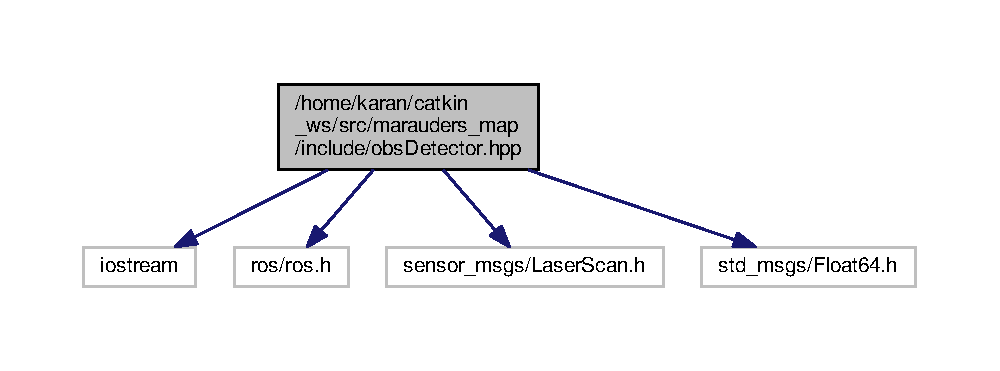
\includegraphics[width=350pt]{obs_detector_8hpp__incl}
\end{center}
\end{figure}
This graph shows which files directly or indirectly include this file\+:
\nopagebreak
\begin{figure}[H]
\begin{center}
\leavevmode
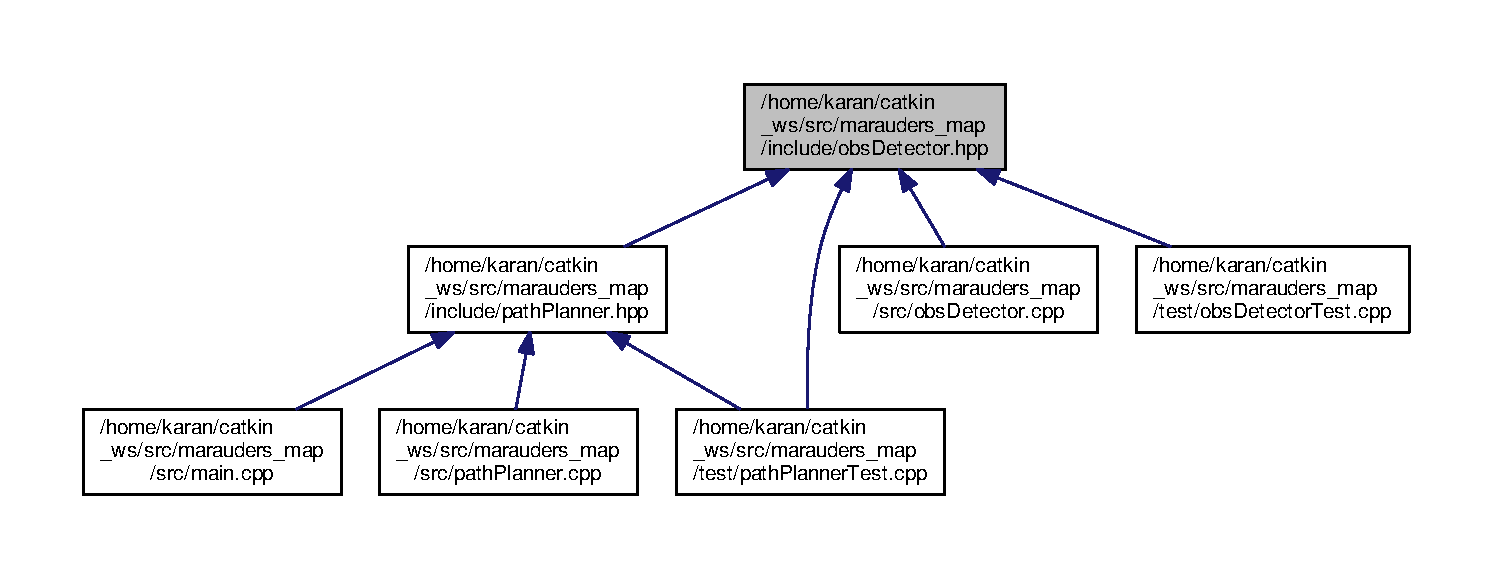
\includegraphics[width=350pt]{obs_detector_8hpp__dep__incl}
\end{center}
\end{figure}
\subsection*{Classes}
\begin{DoxyCompactItemize}
\item 
class \hyperlink{class_obs_detector}{Obs\+Detector}
\begin{DoxyCompactList}\small\item\em Class for \hyperlink{class_obs_detector}{Obs\+Detector}. \end{DoxyCompactList}\end{DoxyCompactItemize}


\subsection{Detailed Description}
Final Project -\/ Marauders Map -\/ Mapping an unknown environment. 

M\+IT License

Copyright (c) 2017 Karan Vivek Bhargava

Permission is hereby granted, free of charge, to any person obtaining a copy of this software and associated documentation files (the \char`\"{}\+Software\char`\"{}), to deal in the Software without restriction, including without limitation the rights to use, copy, modify, merge, publish, distribute, sublicense, and/or sell copies of the Software, and to permit persons to whom the Software is furnished to do so, subject to the following conditions\+:

The above copyright notice and this permission notice shall be included in all copies or substantial portions of the Software.

T\+HE S\+O\+F\+T\+W\+A\+RE IS P\+R\+O\+V\+I\+D\+ED \char`\"{}\+A\+S I\+S\char`\"{}, W\+I\+T\+H\+O\+UT W\+A\+R\+R\+A\+N\+TY OF A\+NY K\+I\+ND, E\+X\+P\+R\+E\+SS OR I\+M\+P\+L\+I\+ED, I\+N\+C\+L\+U\+D\+I\+NG B\+UT N\+OT L\+I\+M\+I\+T\+ED TO T\+HE W\+A\+R\+R\+A\+N\+T\+I\+ES OF M\+E\+R\+C\+H\+A\+N\+T\+A\+B\+I\+L\+I\+TY, F\+I\+T\+N\+E\+SS F\+OR A P\+A\+R\+T\+I\+C\+U\+L\+AR P\+U\+R\+P\+O\+SE A\+ND N\+O\+N\+I\+N\+F\+R\+I\+N\+G\+E\+M\+E\+NT. IN NO E\+V\+E\+NT S\+H\+A\+LL T\+HE A\+U\+T\+H\+O\+RS OR C\+O\+P\+Y\+R\+I\+G\+HT H\+O\+L\+D\+E\+RS BE L\+I\+A\+B\+LE F\+OR A\+NY C\+L\+A\+IM, D\+A\+M\+A\+G\+ES OR O\+T\+H\+ER L\+I\+A\+B\+I\+L\+I\+TY, W\+H\+E\+T\+H\+ER IN AN A\+C\+T\+I\+ON OF C\+O\+N\+T\+R\+A\+CT, T\+O\+RT OR O\+T\+H\+E\+R\+W\+I\+SE, A\+R\+I\+S\+I\+NG F\+R\+OM, O\+UT OF OR IN C\+O\+N\+N\+E\+C\+T\+I\+ON W\+I\+TH T\+HE S\+O\+F\+T\+W\+A\+RE OR T\+HE U\+SE OR O\+T\+H\+ER D\+E\+A\+L\+I\+N\+GS IN T\+HE S\+O\+F\+T\+W\+A\+RE.

\begin{DoxyAuthor}{Author}
Karan Vivek Bhargava 
\end{DoxyAuthor}
\begin{DoxyCopyright}{Copyright}
M\+IT License
\end{DoxyCopyright}
\hypertarget{path_planner_8cpp_DESCRIPTION}{}\subsection{D\+E\+S\+C\+R\+I\+P\+T\+I\+ON}\label{path_planner_8cpp_DESCRIPTION}
This program will perform laserscan for the turtlebot to check for collisions 
\hypertarget{path_planner_8hpp}{}\section{/home/karan/catkin\+\_\+ws/src/marauders\+\_\+map/include/path\+Planner.hpp File Reference}
\label{path_planner_8hpp}\index{/home/karan/catkin\+\_\+ws/src/marauders\+\_\+map/include/path\+Planner.\+hpp@{/home/karan/catkin\+\_\+ws/src/marauders\+\_\+map/include/path\+Planner.\+hpp}}


Final Project -\/ Marauders Map -\/ Mapping an unknown environment.  


{\ttfamily \#include \char`\"{}geometry\+\_\+msgs/\+Twist.\+h\char`\"{}}\\*
{\ttfamily \#include \char`\"{}obs\+Detector.\+hpp\char`\"{}}\\*
Include dependency graph for path\+Planner.\+hpp\+:
\nopagebreak
\begin{figure}[H]
\begin{center}
\leavevmode
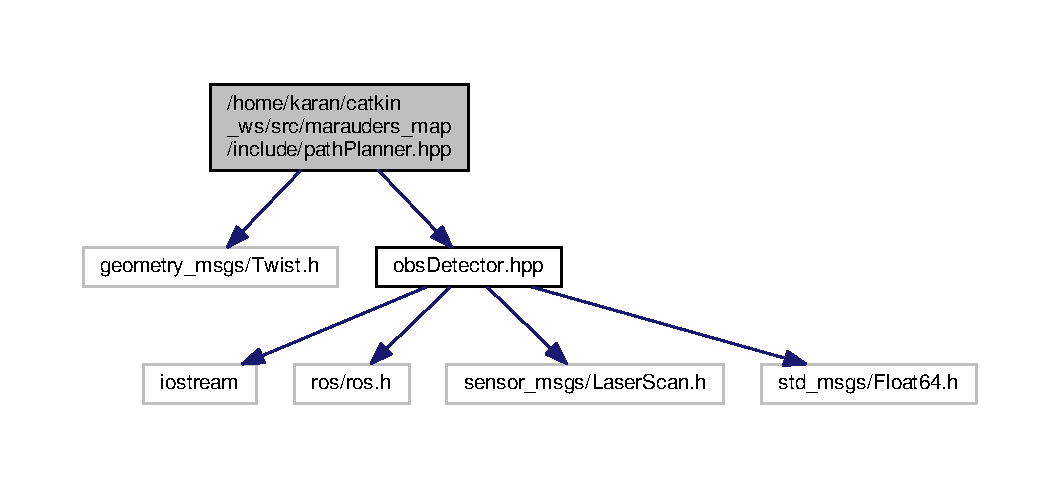
\includegraphics[width=350pt]{path_planner_8hpp__incl}
\end{center}
\end{figure}
This graph shows which files directly or indirectly include this file\+:
\nopagebreak
\begin{figure}[H]
\begin{center}
\leavevmode
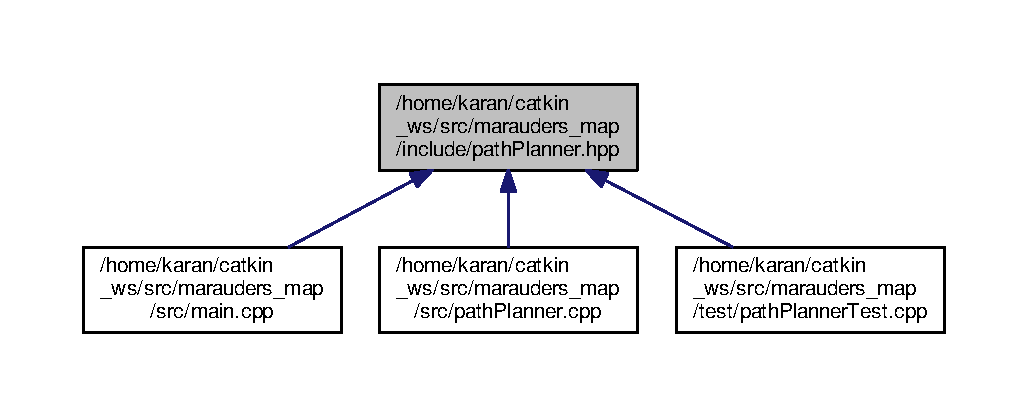
\includegraphics[width=350pt]{path_planner_8hpp__dep__incl}
\end{center}
\end{figure}
\subsection*{Classes}
\begin{DoxyCompactItemize}
\item 
class \hyperlink{class_path_planner}{Path\+Planner}
\begin{DoxyCompactList}\small\item\em Class for \hyperlink{class_path_planner}{Path\+Planner}. \end{DoxyCompactList}\end{DoxyCompactItemize}


\subsection{Detailed Description}
Final Project -\/ Marauders Map -\/ Mapping an unknown environment. 

M\+IT License

Copyright (c) 2017 Karan Vivek Bhargava

Permission is hereby granted, free of charge, to any person obtaining a copy of this software and associated documentation files (the \char`\"{}\+Software\char`\"{}), to deal in the Software without restriction, including without limitation the rights to use, copy, modify, merge, publish, distribute, sublicense, and/or sell copies of the Software, and to permit persons to whom the Software is furnished to do so, subject to the following conditions\+:

The above copyright notice and this permission notice shall be included in all copies or substantial portions of the Software.

T\+HE S\+O\+F\+T\+W\+A\+RE IS P\+R\+O\+V\+I\+D\+ED \char`\"{}\+A\+S I\+S\char`\"{}, W\+I\+T\+H\+O\+UT W\+A\+R\+R\+A\+N\+TY OF A\+NY K\+I\+ND, E\+X\+P\+R\+E\+SS OR I\+M\+P\+L\+I\+ED, I\+N\+C\+L\+U\+D\+I\+NG B\+UT N\+OT L\+I\+M\+I\+T\+ED TO T\+HE W\+A\+R\+R\+A\+N\+T\+I\+ES OF M\+E\+R\+C\+H\+A\+N\+T\+A\+B\+I\+L\+I\+TY, F\+I\+T\+N\+E\+SS F\+OR A P\+A\+R\+T\+I\+C\+U\+L\+AR P\+U\+R\+P\+O\+SE A\+ND N\+O\+N\+I\+N\+F\+R\+I\+N\+G\+E\+M\+E\+NT. IN NO E\+V\+E\+NT S\+H\+A\+LL T\+HE A\+U\+T\+H\+O\+RS OR C\+O\+P\+Y\+R\+I\+G\+HT H\+O\+L\+D\+E\+RS BE L\+I\+A\+B\+LE F\+OR A\+NY C\+L\+A\+IM, D\+A\+M\+A\+G\+ES OR O\+T\+H\+ER L\+I\+A\+B\+I\+L\+I\+TY, W\+H\+E\+T\+H\+ER IN AN A\+C\+T\+I\+ON OF C\+O\+N\+T\+R\+A\+CT, T\+O\+RT OR O\+T\+H\+E\+R\+W\+I\+SE, A\+R\+I\+S\+I\+NG F\+R\+OM, O\+UT OF OR IN C\+O\+N\+N\+E\+C\+T\+I\+ON W\+I\+TH T\+HE S\+O\+F\+T\+W\+A\+RE OR T\+HE U\+SE OR O\+T\+H\+ER D\+E\+A\+L\+I\+N\+GS IN T\+HE S\+O\+F\+T\+W\+A\+RE.

\begin{DoxyAuthor}{Author}
Karan Vivek Bhargava 
\end{DoxyAuthor}
\begin{DoxyCopyright}{Copyright}
M\+IT License
\end{DoxyCopyright}
\hypertarget{path_planner_8cpp_DESCRIPTION}{}\subsection{D\+E\+S\+C\+R\+I\+P\+T\+I\+ON}\label{path_planner_8cpp_DESCRIPTION}
This program will perform path planning operations for the turtlebot to check for collisions 
\hypertarget{obs_detector_8cpp}{}\section{/home/karan/catkin\+\_\+ws/src/marauders\+\_\+map/src/obs\+Detector.cpp File Reference}
\label{obs_detector_8cpp}\index{/home/karan/catkin\+\_\+ws/src/marauders\+\_\+map/src/obs\+Detector.\+cpp@{/home/karan/catkin\+\_\+ws/src/marauders\+\_\+map/src/obs\+Detector.\+cpp}}


Final Project -\/ Marauders Map -\/ Mapping an unknown environment.  


{\ttfamily \#include \char`\"{}obs\+Detector.\+hpp\char`\"{}}\\*
Include dependency graph for obs\+Detector.\+cpp\+:
\nopagebreak
\begin{figure}[H]
\begin{center}
\leavevmode
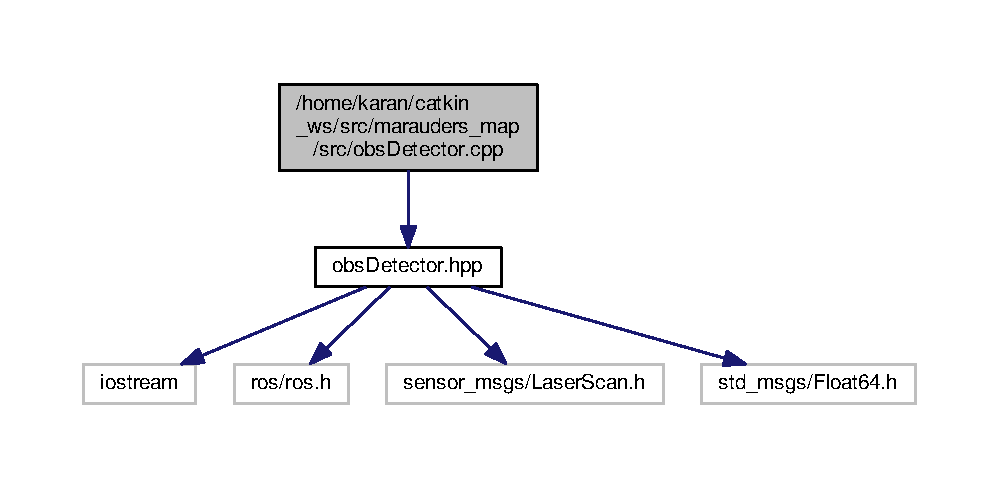
\includegraphics[width=350pt]{obs_detector_8cpp__incl}
\end{center}
\end{figure}


\subsection{Detailed Description}
Final Project -\/ Marauders Map -\/ Mapping an unknown environment. 

M\+IT License

Copyright (c) 2017 Karan Vivek Bhargava

Permission is hereby granted, free of charge, to any person obtaining a copy of this software and associated documentation files (the \char`\"{}\+Software\char`\"{}), to deal in the Software without restriction, including without limitation the rights to use, copy, modify, merge, publish, distribute, sublicense, and/or sell copies of the Software, and to permit persons to whom the Software is furnished to do so, subject to the following conditions\+:

The above copyright notice and this permission notice shall be included in all copies or substantial portions of the Software.

T\+HE S\+O\+F\+T\+W\+A\+RE IS P\+R\+O\+V\+I\+D\+ED \char`\"{}\+A\+S I\+S\char`\"{}, W\+I\+T\+H\+O\+UT W\+A\+R\+R\+A\+N\+TY OF A\+NY K\+I\+ND, E\+X\+P\+R\+E\+SS OR I\+M\+P\+L\+I\+ED, I\+N\+C\+L\+U\+D\+I\+NG B\+UT N\+OT L\+I\+M\+I\+T\+ED TO T\+HE W\+A\+R\+R\+A\+N\+T\+I\+ES OF M\+E\+R\+C\+H\+A\+N\+T\+A\+B\+I\+L\+I\+TY, F\+I\+T\+N\+E\+SS F\+OR A P\+A\+R\+T\+I\+C\+U\+L\+AR P\+U\+R\+P\+O\+SE A\+ND N\+O\+N\+I\+N\+F\+R\+I\+N\+G\+E\+M\+E\+NT. IN NO E\+V\+E\+NT S\+H\+A\+LL T\+HE A\+U\+T\+H\+O\+RS OR C\+O\+P\+Y\+R\+I\+G\+HT H\+O\+L\+D\+E\+RS BE L\+I\+A\+B\+LE F\+OR A\+NY C\+L\+A\+IM, D\+A\+M\+A\+G\+ES OR O\+T\+H\+ER L\+I\+A\+B\+I\+L\+I\+TY, W\+H\+E\+T\+H\+ER IN AN A\+C\+T\+I\+ON OF C\+O\+N\+T\+R\+A\+CT, T\+O\+RT OR O\+T\+H\+E\+R\+W\+I\+SE, A\+R\+I\+S\+I\+NG F\+R\+OM, O\+UT OF OR IN C\+O\+N\+N\+E\+C\+T\+I\+ON W\+I\+TH T\+HE S\+O\+F\+T\+W\+A\+RE OR T\+HE U\+SE OR O\+T\+H\+ER D\+E\+A\+L\+I\+N\+GS IN T\+HE S\+O\+F\+T\+W\+A\+RE.

\begin{DoxyAuthor}{Author}
Karan Vivek Bhargava 
\end{DoxyAuthor}
\begin{DoxyCopyright}{Copyright}
M\+IT License
\end{DoxyCopyright}
\hypertarget{path_planner_8cpp_DESCRIPTION}{}\subsection{D\+E\+S\+C\+R\+I\+P\+T\+I\+ON}\label{path_planner_8cpp_DESCRIPTION}
This program will perform laserscan for the turtlebot to check for collisions 
\hypertarget{path_planner_8cpp}{}\section{/home/karan/catkin\+\_\+ws/src/marauders\+\_\+map/src/path\+Planner.cpp File Reference}
\label{path_planner_8cpp}\index{/home/karan/catkin\+\_\+ws/src/marauders\+\_\+map/src/path\+Planner.\+cpp@{/home/karan/catkin\+\_\+ws/src/marauders\+\_\+map/src/path\+Planner.\+cpp}}


Final Project -\/ Marauders Map -\/ Mapping an unknown environment.  


{\ttfamily \#include \char`\"{}path\+Planner.\+hpp\char`\"{}}\\*
Include dependency graph for path\+Planner.\+cpp\+:
\nopagebreak
\begin{figure}[H]
\begin{center}
\leavevmode
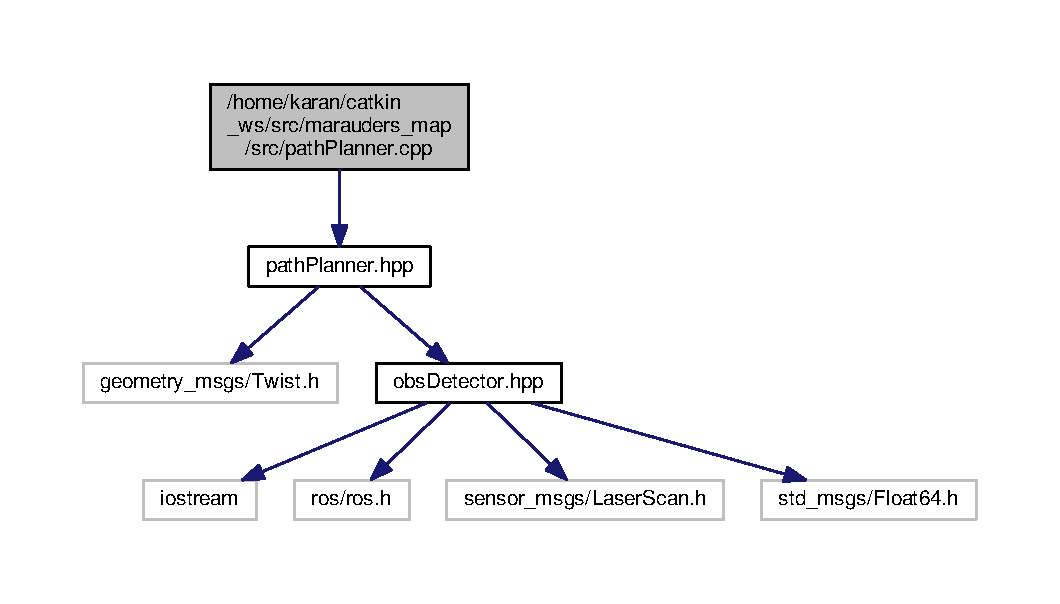
\includegraphics[width=350pt]{path_planner_8cpp__incl}
\end{center}
\end{figure}


\subsection{Detailed Description}
Final Project -\/ Marauders Map -\/ Mapping an unknown environment. 

M\+IT License

Copyright (c) 2017 Karan Vivek Bhargava

Permission is hereby granted, free of charge, to any person obtaining a copy of this software and associated documentation files (the \char`\"{}\+Software\char`\"{}), to deal in the Software without restriction, including without limitation the rights to use, copy, modify, merge, publish, distribute, sublicense, and/or sell copies of the Software, and to permit persons to whom the Software is furnished to do so, subject to the following conditions\+:

The above copyright notice and this permission notice shall be included in all copies or substantial portions of the Software.

T\+HE S\+O\+F\+T\+W\+A\+RE IS P\+R\+O\+V\+I\+D\+ED \char`\"{}\+A\+S I\+S\char`\"{}, W\+I\+T\+H\+O\+UT W\+A\+R\+R\+A\+N\+TY OF A\+NY K\+I\+ND, E\+X\+P\+R\+E\+SS OR I\+M\+P\+L\+I\+ED, I\+N\+C\+L\+U\+D\+I\+NG B\+UT N\+OT L\+I\+M\+I\+T\+ED TO T\+HE W\+A\+R\+R\+A\+N\+T\+I\+ES OF M\+E\+R\+C\+H\+A\+N\+T\+A\+B\+I\+L\+I\+TY, F\+I\+T\+N\+E\+SS F\+OR A P\+A\+R\+T\+I\+C\+U\+L\+AR P\+U\+R\+P\+O\+SE A\+ND N\+O\+N\+I\+N\+F\+R\+I\+N\+G\+E\+M\+E\+NT. IN NO E\+V\+E\+NT S\+H\+A\+LL T\+HE A\+U\+T\+H\+O\+RS OR C\+O\+P\+Y\+R\+I\+G\+HT H\+O\+L\+D\+E\+RS BE L\+I\+A\+B\+LE F\+OR A\+NY C\+L\+A\+IM, D\+A\+M\+A\+G\+ES OR O\+T\+H\+ER L\+I\+A\+B\+I\+L\+I\+TY, W\+H\+E\+T\+H\+ER IN AN A\+C\+T\+I\+ON OF C\+O\+N\+T\+R\+A\+CT, T\+O\+RT OR O\+T\+H\+E\+R\+W\+I\+SE, A\+R\+I\+S\+I\+NG F\+R\+OM, O\+UT OF OR IN C\+O\+N\+N\+E\+C\+T\+I\+ON W\+I\+TH T\+HE S\+O\+F\+T\+W\+A\+RE OR T\+HE U\+SE OR O\+T\+H\+ER D\+E\+A\+L\+I\+N\+GS IN T\+HE S\+O\+F\+T\+W\+A\+RE.

\begin{DoxyAuthor}{Author}
Karan Vivek Bhargava 
\end{DoxyAuthor}
\begin{DoxyCopyright}{Copyright}
M\+IT License
\end{DoxyCopyright}
\hypertarget{path_planner_8cpp_DESCRIPTION}{}\subsection{D\+E\+S\+C\+R\+I\+P\+T\+I\+ON}\label{path_planner_8cpp_DESCRIPTION}
This program will perform laserscan for the turtlebot to check for collisions 
%--- End generated contents ---

% Index
\backmatter
\newpage
\phantomsection
\clearemptydoublepage
\addcontentsline{toc}{chapter}{Index}
\printindex

\end{document}
